% Changing book to article will make the footers match on each page,
% rather than alternate every other.
%
% Note that the article class does not have chapters.
\documentclass[10pt,twoside,twocolumn,openany]{book}
\usepackage[bg-letter]{dnd} % Options: bg-a4, bg-letter, bg-full, bg-print, bg-none.
\usepackage[english]{babel}
\usepackage[utf8]{inputenc}
\usepackage{graphicx}
% Start document
\begin{document}
\fontfamily{ppl}\selectfont % Set text font

% Your content goes here

% Comment this out if you're using the article class.
\chapter{Hyrule Races}

\section{Goron}

\subsection{Physiology}
Gorons stand taller and wider than hylians, and universally have skin of an orange-brown hue. What little "hair" they possess is so stiff and thick it resembles solid rock, and usually grows only high on a goron's scalp and across its upper back. A few gorons are also able to grow beards or other facial hair, especially if they are of advanced age. A pair of goron eyes are wide set, perfectly circular, and completely dark—posessing no whites like those of a hylian's or gerudo's eyes. Goron noses are flat. Jaws are very wide, powerful, and composed entirely of molars—used to crush and pulverize the rocks which famously make up goron diets.\\
Although they are physiologically more similar to earth elementals than mammals, gorons nonetheless take a humanoid shape. They are required to eat and sleep to live. Drinking serves no purpose for them. They can persist indefinitely without breathing, but doing so is unpleasant, especially when the goron is exerting itself. Mysteriously, gorons dine on rocks and other solid minerals—tastes vary between tribes, as some prefer coarse ores, others savor gemstones, but they generally dislike less solid earth such as sand or dirt. A few dine on more traditional foods such as meat or mushrooms, but this seems to be for pleasure rather than sustenance.\\
Because they are literally made of rock, gorons have an inherent durability to their bodies, but are also particularly dense and heavy. This makes traditional movement difficult for them over anything but short distances. When traveling more than a few feet, a goron will usually tuck itself into a ball and roll, which allows it to traverse ground at much greater speed. This speed of this "goron roll" combined with a goron's weight makes it a powerful charging attack for chasing down foes. Aside from this, gorons battle with powerful punches—punches so powerful that fighting unarmed is the norm among their race.\\
Gorons only possess one apparent sex, which they universally refer to as male. "Brother" is a very common term of endearment among them, and friends of a goron tribe are often referred to as brothers—regardless of whether or not they are male.

\subsection{Society}
Goron cities and villages are almost universally built into caves or the sides of mountains, where the tastiest and most nutritious rocks are abundant. Their reliance on 
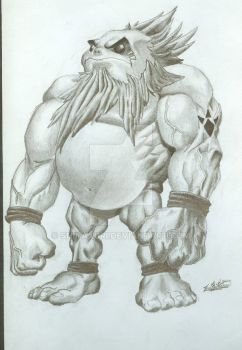
\includegraphics{darunia.jpg} \\
eating rocks makes their cultures particularly dependent on mining to survive, to the extent that the majority of gorons have experience in this profession. Many anthropologists believe gorons evolved to be as physically powerful and enduring as they are due to their race's inherent dependency on mining. Stronger gorons with greater strength made better miners, which enabled them to better survive and provide for their kin.\\
Due to their mining dependency, goron culture heavily involves stonework and the working of metals. Blacksmiths are abundant among them, and their structures are constructed almost entirely of metal. They're also one of few races that has widely adapted the use of blackpowder, and when in battle they often make use of bombs or other explosives. Their resistance to heat gives them an edge over most foes when using such powerful, but esoteric weapons.\\
Gorons almost always place a high degree of value on physical strength and stamina, pride, honesty, and trustworthiness. Gorons most readily get along with races which share these values, usually including the like of subrosians, rito, and most hylians. A friend is rarely lost on a goron unless that friend is caught in a lie. Unsurprisingly, gorons often have a difficult time with people from less prideful cultures.

\subsection{Goron Names}
Goron names are all considered male. These names more often than not consist of at least one "go" or "da" syllable. Deep vowel sounds such as "ah," "oh," and "oo" are prominent. "R" consonants are also very common, especially in the center of the name. \\
\textbf{Male:} Biggoron, Darbus, Daruk, Darmani, Darunia, Gongoron, Gorko, Gortram, Kabetta, Kagoron, Medigoron, Reagah, Rohan, Tanko, Volcon, Yunobo. 

\subsection{Goron Traits}
Built like mountains, eating rocks, and wading through lava — gorons are nothing if not hardy and impregnable.
\indent \textbf{Ability Score Increase.} Your Strength score increases by 2 and your Constitution scores increases by 1.\\
\indent \textbf{Age.} Gorons reach adulthood in about a decade, but can live to be over a century. \\
\indent \textbf{Alignment.} Although gorons can alienate those outside their kin group, they form strong bonds with those they trust. They have a tendency towards lawful good.\\
\indent \textbf{Size.} Gorons are usually between 6 and 8 feet in height, and quite stocky. Your size is Medium.\\
\indent \textbf{Speed.} Your base walking speed is 25 feet.\\
\indent \textbf{Hot Skin.} You have advantage on saving throws against fire damage, resistance to fire damage, and are unable to catch flame. On the other hand, you have disadvantage on all saving throws against cold damage.\\
\indent \textbf{Stone Armor.} Your skin is hard as stone. When you aren’t wearing armor and not wielding a shield, your AC is 13 + your Constitution modifier.\\
\indent \textbf{Darkvision.} Accustomed to life underground, you have superior vision in dark and dim conditions. You can see in dim light within 60 feet of you as if it were bright light, and in darkness as if it were dim light. You can’t discern color in darkness, only shades of gray.\\
\indent \textbf{Natural Athlete.} You are proficient in the Athletics skill.\\
\indent \textbf{Like Stone.} You can attempt to hide when you are surrounded by any kind of rocky terrain. Additionally, you can move across difficult terrain made of earth or stone without expending extra movement.\\
\indent \textbf{Stone in the Water.} You sink to the bottom of any body of water you enter. Also, you have no need to drink water, and can hold your breath indefinitely. While underwater, you have disadvantage on all ability checks and attack rolls.\\
\indent \textbf{Goron Roll.} When you take the Dash action, you gain the extra movement you otherwise would plus 20. If you take the Dash action and move at least 20 feet straight towards a creature, you can make a roll attack against that creature as a bonus action. This attack counts as an unarmed strike against the target and its damage is decided by a d4 dice roll plus your Strength modifier. This dice changes as you level up, as shown in the Roll Attack table. 
\begin{dndtable}
 	\textbf{Goron Level}  & \textbf{Roll Attack Damage} \\
    1st  & 1d4 + Strength Modifier \\
 	5th  & 1d6 + Strength Modifier\\
  	11th  & 1d8 + Strength Modifier\\
    17th  & 1d10 + Strength Modifier\\
\end{dndtable}
\indent \textbf{Rock Gourmet.} You are able to eat half a pound of rock instead of consuming a portion of rations whenever you feel hungry.\\
\indent \textbf{Languages.} You can speak, read, and write Common and Goro.
\newpage
\section{Zora}

\subsection{Physiology}

Amphibious, fish-like humanoids, zora have sleek and glistening bodies. Zora rarely breed, but when they do, they have offspring in batches of eggs ranging from 1 to 8, which grow into tadpoles, and eventually amphibious humanoids. Zora age at a slow rate compared to hylians, but have a growth spurt and reach adulthood around the age of 20, reach middle age at about 100 years, and can occasionally live to be more than 200.
The exact shape and demeanor of zora is heavily dependent on the two subraces: sea zora, and river zora. "Sea zora" have evolved to live in deeper saltwater, and "river zora" have evolved to live in shallower freshwater, but modern zora of either variety can be found in either habitat.\\
Sea zora are taller and more slender, and have a pale white chest and face, with a backside of a darker color—usually blue, but occasionally red, gray, brown, or other colors. The shape of a sea zora's head varies widely, but usually has a backside resembling some variety of fish tail, with fins that further aid its ability to swim.\\
River zora are squatter and wider, though still slightly larger than hylians on average. Their scales are a blush-green color that blends well into seaweed and shallow rivers, but their heads feature orange fins and lips.

\subsection{Society}

Due to their amphibious nature, zora villages are most often built along coastlines, rivers, lakes, and other areas that blend shallow water with nearby land. This enables them to effectively evade and defend against predators that are exclusive to land or sea, and hunt more effectively from both sources. Zora usually wear a small amount of jewelry or armor, but less clothing than races such as hylians or rito, as excess clothing hampers their ability to swim.\\
A given zora tribe is usually ruled by a royal family of zora, to which the tribe is loyal for generations. The current monarch of a tribe is often referred to with a title such as "King Zora" or "Queen Zora" than his or her actual name.\\
River zora are more hostile to outside races, including sea zora. They have an instinctive desire to aggressively defend what waters they call their own, and will attack any foreign entities with blasts of fire without hesitation. The rare outsider who can gain the trust of a river zora tribe will find they are not murderers nor thieves, but are in fact quite friendly to their allies.\\
Sea zora are comparatively more accepting, and their royal families are usually allies with the royal families of hylians. They frequently intermingle with other races who live on coastlines, and are renowned for their unique \\
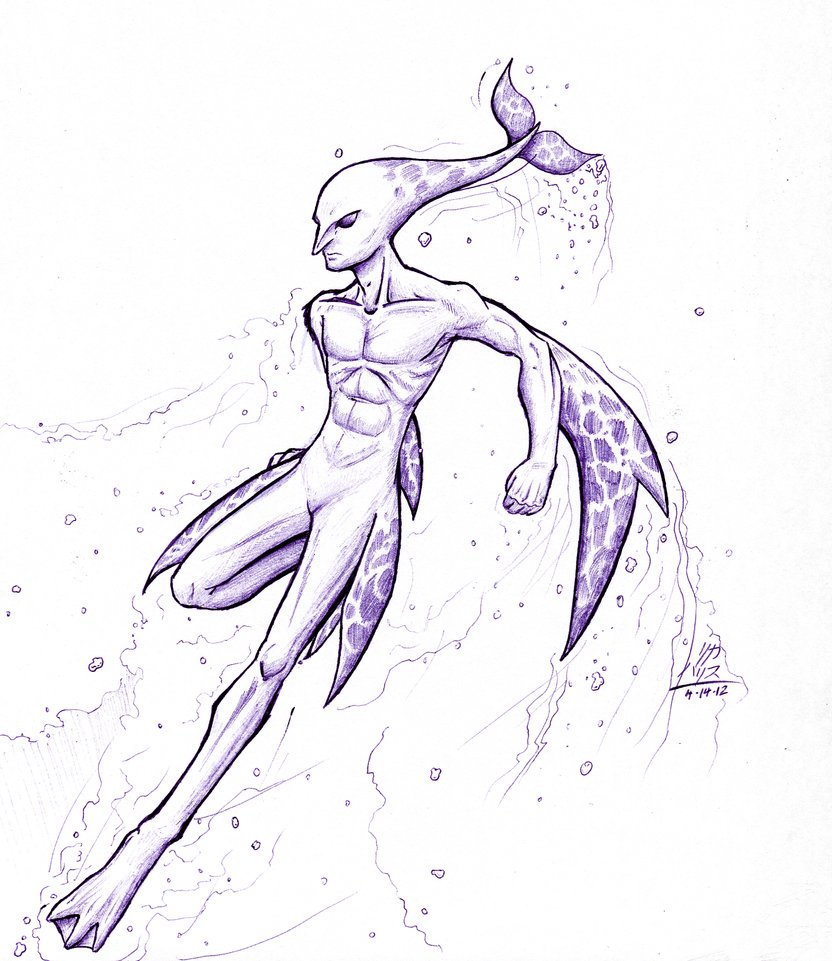
\includegraphics{zora.png} \\
style of music.

\subsection{Zora Names}

\textbf{Male:} Cleff, Japas, Mikau, Ralis, Sidon, Tijo, Toto \\
\textbf{Female:} Laruto, Lulu, Mipha, Oren, Rutela, Ruto 

\subsection{Zora Traits}
Zora claim the title of the only truly amphibious race in Hyrule — and are the second most populous, exceeded only by hylians.\\
\indent \textbf{Ability Score Increase.} Your Wisdom score increases by 2 and your Dexterity score increases by 1.\\
\indent \textbf{Age.} Zora reach adulthood by the age of 20 at the earliest, and can live to an age of 200 or more.\\
\indent \textbf{Alignment.} Zora tend towards lawful neutral.\\
\indent \textbf{Size.} A zora can vary greatly in size, but is usually about 6 feet tall. Rarely, a zora can grow to a height of 8 feet or more. Your size is Medium.\\
\indent \textbf{Speed.} Your base walking speed is 30 feet, and you have a swim speed of 60 feet.\\
\indent \textbf{Amphibious.} You can breathe both air and water.\\
\indent \textbf{Underwater Camouflage.} When you make a Dexterity (Stealth) check while mostly or entirely underwater, you do so with advantage. \\
\indent \textbf{One with the Water.} You have advantage on all Acrobatics, Animal Handling, Nature and Survival ability checks that involve water or any animal that lives in a wet environment.\\
\indent \textbf{Fire Vulnerability.} You are vulnerable to fire damage attacks.\\
\indent \textbf{Keen Senses.} You have proficiency in the Perception skill.\\
\indent \textbf{Lightning Field.} You can cast the lightning field cantrip. Wisdom is your casting ability for this spell. \\
\indent \textbf{Ancestral Arms.} You have proficiency with the arm blade, pike, net, spear, and trident. If you otherwise gain proficiency with spears or tridents, you gain a +1 bonus on damage rolls with these weapons.\\
\indent \textbf{Languages.} You can speak, write, and read Common and Zoran.

\chapter{Hyrule Spells}
%The spells are presented in alphabetical order.

\section{Lightning Field}
\textit{Evocation Cantrip} \\

\noindent \textbf{Casting Time:} 1 action\\
\textbf{Range:} 5 feet\\
\textbf{Components:} S\\
\textbf{Duration:} Instantaneous\\

\noindent A cylindrical aura of electricity sweeps around you for a moment, jolting adjacent foes. Each creature within range, other than you, must succeed on a Dexterity saving throw or take 1d6 lightning damage. \\
This spell's damage increases by 1d6 when you reach 5th level (2d6), 11th level (3d6), and 17th level (4d6). \\

%\begin{commentbox}{Neat Green Box!}
%	\lipsum[1]
%\end{commentbox}

%\subtitlesection{Weapon, +1, +2, or +3}
%{Weapon (any), uncommon (+1), rare (+2), or very rare (+3)}

%\begin{quotebox}
%	As you approach this template you get a sense that the blood and tears of many generations went into its making. A warm feeling welcomes you as you type your first words.
%\end{quotebox}

%\newpage % Acts as columbreak because of twocolumn option; for pagebreak use \clearpage

% For more columns, you can say \begin{dndtable}[your options here}.
% For instance, if you wanted three columns, you could say
% \begin{dndtable}{XXX}. The usual host of tabular parameters are
% aailable as well.
%\header{Nice table}


%\begin{paperbox}{Do the Players need direction?}
%	\lipsum[1]
%\end{paperbox}

% You can optionally not include the background by saying
% begin{monsterboxnobg}
\begin{comment}
\begin{monsterbox}{Monster Foo}
	\textit{Small metasyntactic variable (goblinoid), neutral evil}\\
	\hline
	\basics[%
	armorclass = 12,
	hitpoints  = 16 (3d8 + 3),
	speed      = 50 ft
	]
	\hline
	\stats[
    STR = \stat{12}, % This stat command will autocomplete the modifier for you
    DEX = \stat{7}
	]
	\hline
	\details[%
	% If you want to use commas in these sections, enclose the
	% description in braces.
	% I'm so sorry.
	languages = {Common Lisp, Erlang},
	]
	\hline \\[1mm]
	\begin{monsteraction}[Monster-super-powers]
		This Monster has some serious superpowers!
	\end{monsteraction}
	\monstersection{Actions}
	\begin{monsteraction}[Generate text]
		This one can generate tremendous amounts of text! Though only when it wants to.
	\end{monsteraction}

	\begin{monsteraction}[More actions]
    See, here he goes again! Yet more text.
	\end{monsteraction}
\end{monsterbox}
\end{comment}
% End document
\end{document}
